%!TEX encoding = UTF-8 Unicode
\documentclass[master,korean,final]{cbnu-ecs}

% kaist.cls 에서는 기본으로 dhucs, ifpdf, graphicx 패키지가 로드됩니다.
% 추가로 필요한 패키지가 있다면 주석을 풀고 적어넣으십시오,
%\usepackage{...}
%

%\usepackage{kotex}
\usepackage{multirow}
\usepackage{varwidth}
\usepackage{amsmath}
\usepackage{indentfirst}
\usepackage{algorithm,algpseudocode}
\usepackage{booktabs}
\usepackage{longtable}

%\renewcommand\tablename{표}
%\renewcommand\figurename{그림}

\newtheorem{theorem}{Theorem}	

% @command title 논문 제목
% @options [default: (none)]
% - korean: 한글제목 | english: 영문제목
\title[korean]{선분 카메라쌍 알고리즘을 이용한 사각형 특징의 기하학적 자세 추정을 통한 Factor Graph 기반 비주얼 SLAM}
\title[english]{Factor Graph based Visual SLAM with Geometric Pose Estimation of a Rectangle Feature using Coupled Line Camera Algorithm}

\author[korean] {이}{재 민}
\author[english]{Lee}{Jae min}

\advisor[major]{박 찬 식}{Chan sik Park}{signed}

\department{RO}

% @command studentid 학번
\studentid{2014298010}

% 논문제출일
\submitdate{2016}{4}{1}

% @command approvaldate 지도교수논문승인일
% @param   year,month,day 연,월,일 순으로 입력
\approvaldate{2016}{6}{15}

% @command refereedate 심사위원논문심사일
% @param   year,month,day 연,월,일 순으로 입력
\refereedate{2016}{6}{1}

% @command gradyear 졸업년도
\gradyear{2016}{8}

% 본문 시작
\begin{document}

% 목차 (Table of Contents) 생성
\tableofcontents

% 영문초록 (abstract)
\begin{abstract}
Modern networks are large-scale, composed of many layers with tens of thousands of devices. 
Cloud computing data centers and multi-layered transport networks are 
examples of such networks.
\ldots
\end{abstract}

% 표목차 (List of Tables) 생성
\listoftables

% 그림목차 (List of Figures) 생성
\listoffigures

% 위의 세 종류의 목차는 한꺼번에 다음 명령으로 생성할 수도 있습니다.
%\makecontents

\pagenumbering{arabic}

\chapter{서론}
\begin{figure}[!ht]
  \centering
	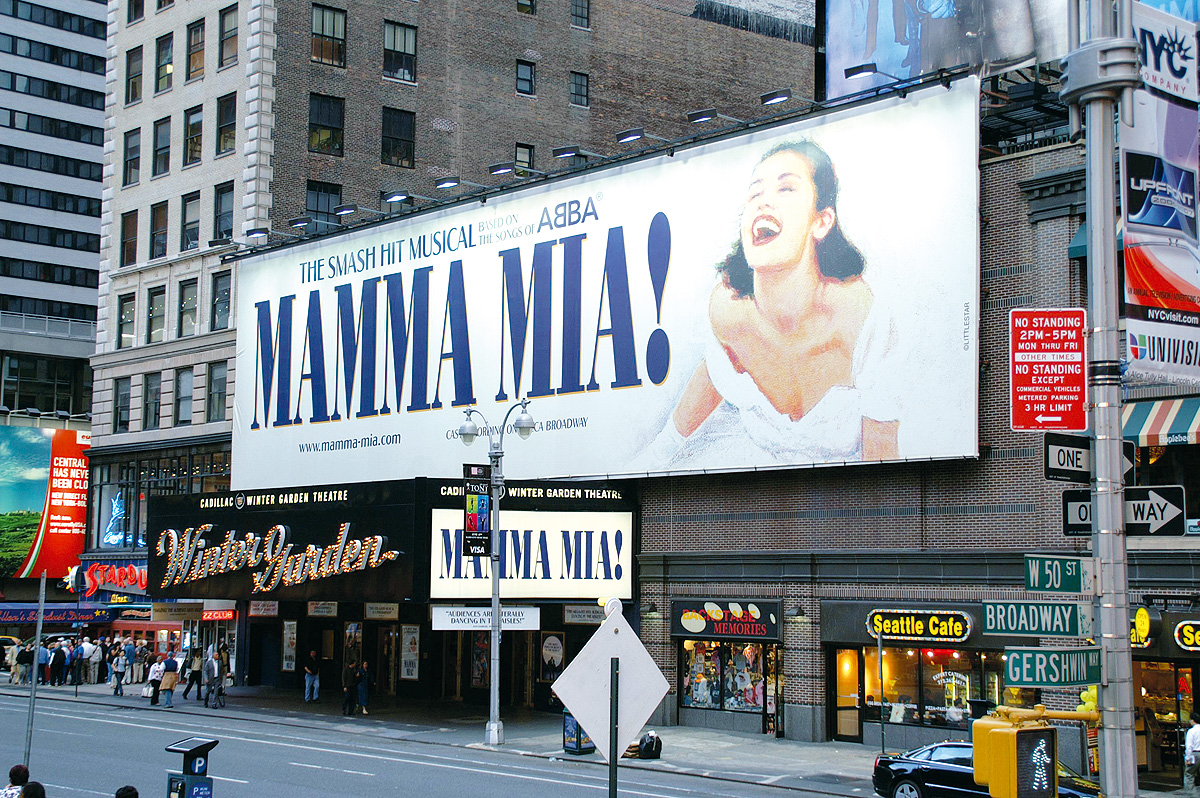
\includegraphics[width=360px]{img/BroadwayPlayers_01.jpg}
  \caption{A picture of the same gull looking the other way!}
\end{figure}
aaa\cite{Davison2007}
%\fontsize{11}{20.5}\selectfont

\section{연구 동기}
zkzkz
\section{관련 연구}
\section{사각형 특징을 활용한 종래 연구}
\chapter{사각형 특징 추출(segmentation)}
\chapter{사각형 특징 기반 Visual SLAM}
\section{자세 추정을 위한 사각형 복원 방법}
\subsection{선분 카메라쌍 방법을 이용한 사각형 복원 방법}
\subsection{3차원 자세 추정을 위한 스테레오 카메라 기반의 선분카메라쌍 방법}
\section{FactorGraphSLAM}
\subsection{}
\chapter{Data Association}
\chapter{Feature Desctiption}
\chapter{실험결과}
\section{CLC Pose estimation validation}
\section{Room/indoor robot test}
\section{Outdoor(Campus) test}
\section{Public Dataset}
\section{Descriptor Test}
\chapter{결론}


\chapter{실험결과}

본 논문에서 제안하는 방법의 타당성을 평가하기위해 몇가지 실험을 통해 입증한다. \\
asdasda\\
asdasd\\
asdasda
sdas

\chapter{결론}

dd


% references section

% can use a bibliography generated by BibTeX as a .bbl file
% BibTeX documentation can be easily obtained at:
% http://www.ctan.org/tex-archive/biblio/bibtex/contrib/doc/
% The IEEEtran BibTeX style support page is at:
% http://www.michaelshell.org/tex/ieeetran/bibtex/
%\bibliographystyle{IEEEtran}
% argument is your BibTeX string definitions and bibliography database(s)
%\bibliography{IEEEabrv,../bib/paper}
%
% <OR> manually copy in the resultant .bbl file
% set second argument of \begin to the number of references
% (used to reserve space for the reference number labels box)

\bibliographystyle{IEEEtran}%...는 bst 파일의 이름(확장자 없이)
\bibliography{ThesisBibTeX.bib}%...는 bib 파일의 이름(확장자 없이)
%\begin{thebibliography}{1}
%\bibitem{greenberg}
%A. Greenberg, J. Hamilton, D.A. Maltz, and P. Patel,
%\emph{The cost of a Cloud: Research Problems in Data Center Networks},
%ACM SIGCOMM Computer Communication Review (CCR), 
%Vol. 39, No. 1, pp. 68-73, January 2009.
%
%\bibitem{wallin}
%S. Wallin, V. Leijon, 
%\emph{Telecom Network and Service Management: An Operator Survey}, 
%MMNS, 2009.
%
%\bibitem{hscalability}
%Wikipedia, \emph{Horizontal Scalability},
%\url{http://en.wikipedia.org/wiki/Scalability#Scale_horizontally_.28scale_out.29}
%
%\end{thebibliography}


\chapter*{감사의 글}

감사의 글을 적으시면 되겠습니다.
감사합니다.sssss

\begin{flushright}
\vspace{1cm}
이재민 배상
\end{flushright}

\end{document}


